%%%%%%%%%%%%%%%%%%%%%%%%%%%%%%%%%%%%%%%%%%%%%%%%%%%%%%%%%%%%%%%%%%%%%%%%%%%%%%%%%%%%%%%%%%%%%%%%%%%
% Appendix -> Supplementary Tables and Figures of PHLOWER
% Author: Mingbo Cheng
%%%%%%%%%%%%%%%%%%%%%%%%%%%%%%%%%%%%%%%%%%%%%%%%%%%%%%%%%%%%%%%%%%%%%%%%%%%%%%%%%%%%%%%%%%%%%%%%%%%
\chapter{Appendix B: PHLOWER}
\label{chapter:appendixB}

\setstretch{1}

\graphicspath{{appendix/figs}}

\begin{figure}[!ht]
  \centering
  \includegraphics[width=0.95\textwidth]{Fib2Neuron_PHLOWER/fig}
  \vspace{0.1cm}
  \caption[Fibroblasts to Neurons dataset PHLOWER workflow.]{\textbf{Detailed steps of PHLOWER on a single cell data with mouse embryonic fibroblasts towards neurons and myocytes.} \textbf{A)} First, PHLOWER estimates a graph representation using kernels and kamada-kawai layout~\citep{gansner2004graph}.
  Colors corresponds to clusters labels as defined in~\citep{treutlein2016dissecting}. This information (labels) is not used by PHLOWER algorithms \textbf{B)} Next, a pseudo-time is estimated using the zero-order Laplacian and using MEF cluster as root. The definition of a root is the only supervision required in PHLOWER. Edges between cells are obtained via delaunay triangulation (left).  To create holes in the simplical complex, PHLOWER performs a trick by including edges between high pseudo-time towards low pseudo time vertices (middle). If we re-run the graph layout, two holes are clearly visible in the graph. \textbf{C)} PHLOWER next perform the spectral decomposition of the Hodge Laplacian of the simplical complex. This indicates two zero eigen-values (or holes). By plotting eigenvectors values on the edges, we observe that the first eigenvector discriminates edges in the neuornal branch vs. others, while the second eigenvector discriminate the myocyte related cells from others. \textbf{D)} Next, PHLOWER generates trajectories by randon walk on the simplicial complex representation to obtain an edge-flow vectors. \textbf{E)} Finally, PHLOWER creates a trajectory embeding by a dot product of the edge flows with the harmonic decomposition. We observe two clear clusters in the trajectory map (left), which are detected by providing this embeding as input for DBSCAN~\citep{ester1996dbscan}.  We can similarly create a cumulative trajectory map by creating edge flows of trajectories by considering only the first one, two, three and so on first differentiation events. PHLOWER uses this space to delineate backbones of differentiation trajectories and to detect branching points events (in green, right panel). \textbf{F)} PHLOWER outputs a differentiation tree, pseudo-time values and an allocation of cells to positions in the branches. PHLOWER makes use of STREAM to visualise the final trajectories.}
  \label{supfig:fib2neuron-workflow}
\end{figure}

\begin{figure}[!ht]
  \centering
  \includegraphics[width=0.95\textwidth]{toy_harmonic/fig}
  \vspace{0.1cm}
  \caption[Properties of HL decomposition in a graph with holes.]{\textbf{Properties of HL decomposition in a graph with holes.} \emph{Source:~\cite{frantzen2021outlier}}~(modified to fit thesis format and/or clarify key points)}
  \label{supfig:toy-properties}
\end{figure}


\begin{figure}[!ht]
  \centering
  \includegraphics[width=0.95\textwidth]{DLA10_PHLOWER/fig}
  \vspace{0.1cm}
  \caption[Workflow for DLA simulated data.]{\textbf{PHLOWER workflow for the simulated tree dataset with 10 total branches} Panels \textbf{A-F} shown distinct PHLOWER estimates for the simulated data with 10 branches exactly as described in~(\afref{supfig:fib2neuron-workflow}). Note that in this complex multi-branched data, the 2 dimensional representation of the graph layout of the simplicial complex \textbf{B)} can not capture the data complexity and does not properly display all the holes. Clustering analysis in the trajectory embedding detects the six main trajectories present in the data \textbf{E)} and recovers a almost perfect differentiation tree \textbf{F)}. Of note, the number of zero-eigenvalues (10) is higher than the number of main trajectories (6).  This is potentially due to small (and noise associated) holes in the graph. This do not impact the precision of the clustering analysis to find the correct branches.}
  \label{supfig:dla10-workflow}
\end{figure}

\begin{figure}[!ht]
  \centering
  \includegraphics[width=0.95\textwidth]{DLA10/fig}
  \vspace{0.1cm}
  \caption[Differentiation tree backbones in the simulated data with 10 branches.]{\textbf{Differentiation tree backbones in the simulated data with 10 branches.} We present embeddings and trees for the ground truth and 12 evaluated algorithms for a dataset with 10 branches. This dataset has a root branch, three intermediary branches, and six end branches. The colors of cells represent the true labels of branches. Embeddings represent the default output as provided by each algorithm. As this information is not provided by celltree, elpigraph, mst, preode, and slingshot, we used the embedding produced by PHATE29. The same embedding was used to display the ground truth.}
  \label{supfig:dla10}
\end{figure}



\begin{figure}[!ht]
  \centering
  \includegraphics[width=0.75\textwidth]{kidney_QC//fig}
  \vspace{0.1cm}
  \caption[Kidney organoid quality check.]{\textbf{Quality check for kidney organoids single cell data}. We show violin plots with quality check information after filtering and cell detection. These are: \textbf{A)} number of features (genes) in RNA, \textbf{B)} number of counts (transcripts) in RNA, \textbf{C)} proportion of mitochondrial genes (RNA), \textbf{D)} fragment sizes distribution (ATAC), \textbf{E)} number of fragments (ATAC) and \textbf{F)} transcription start site enrichment. All libraries had similar values across days of sampling. }
  \label{supfig:kidney-qc}
\end{figure}

\begin{figure}[!ht]
  \centering
  \includegraphics[width=0.95\textwidth]{kidney_markers//fig}
  \vspace{0.1cm}
        \caption[Kidney branches gene markers.]{\textbf{Kidney branches gene markers}. \textbf{A-E)} Genes markers for kidney branches: Mesoderm, Podocyte, Tubular, Neuron and Stromal. }
  \label{supfig:kidney-markers}
\end{figure}

\begin{figure}[!ht]
  \centering
  \includegraphics[width=0.95\textwidth]{TF_diff//fig}
  \vspace{0.1cm}
        \caption[Regulators associated with cell branches.]{\textbf{Regulators associated with cell branches.} \textbf{A)} Regulators associated with Podocyte cells. We perform a differential expression analysis to find genes specific to podocytes (comparing with tubular cells) (left). Of these DE genes, we select transcription factors, which transcription factor activity (scATAC-seq), is highly correlated with gene expression (middle). Heatmaps display the TF activity and gene expression profiles of these TFs over the differentiation path from mesoderm towards podocyte cells. \textbf{B)} Same as (A) when contrasting tubular cells with podocytes. \textbf{C)} Sames as (A) when contrasting neuronal/muscle cells with all other branches. \textbf{D)} Same as (A) when contrasting stromal cells with all other branches.}
  \label{supfig:TF-diff}
\end{figure}



\begin{figure}[!ht]
  \centering
  \includegraphics[width=0.95\textwidth]{kidney_PHLOWER//fig}
  \vspace{0.1cm}
  \caption[Kidney organoid PHLOWER workflow.]{\textbf{PHLOWER workflow for the kidney organoids data} Panels \textbf{A-F} are obtained as described in~(\afref{supfig:fib2neuron-workflow}). }
  \label{supfig:kidney-workflow}
\end{figure}


\begin{table}[!ht]
\centering
\caption[Friedman-Nemenyi test of TI's structure similarity]{\textbf{Friedman-Nemenyi test of TI's structure similarity.} Asterisks indicate P-values of $<0.05$(*), $<0.01$(**), $<0.001$(***), $<0.0001$(****) obtained via Friedman-Nemenyi test}
\begin{tabular}{rlllllllllll}
  \hline
 & \rotatebox{60}{phlower} &
   \rotatebox{60}{paga\_tree} &
   \rotatebox{60}{monocle3} &
   \rotatebox{60}{raceid\_stemid} &
   \rotatebox{60}{stream} &
   \rotatebox{60}{pcreode} & 
   \rotatebox{60}{tscan} &
   \rotatebox{60}{elpigraph} & 
   \rotatebox{60}{slingshot} &
   \rotatebox{60}{mst} &
   \rotatebox{60}{celltree\_vem} \\
  \hline
paga\_tree &  &  &  &  &  &  &  &  &  &  &  \\
  monocle3 &  &  &  &  &  &  &  &  &  &  &  \\
  raceid\_stemid &  &  &  &  &  &  &  &  &  &  &  \\
  stream &  &  &  &  &  &  &  &  &  &  &  \\
  pcreode & * &  &  &  &  &  &  &  &  &  &  \\
  tscan & * &  &  &  &  &  &  &  &  &  &  \\
  elpigraph & * &  &  &  &  &  &  &  &  &  &  \\
  slingshot & ** &  &  &  &  &  &  &  &  &  &  \\
  mst & **** & * & * &  &  &  &  &  &  &  &  \\
  celltree\_vem & **** & ** & * & * &  &  &  &  &  &  &  \\
  slice & **** & **** & **** & ** & ** & * &  &  &  &  &  \\
   \hline
\end{tabular}
\label{tab:him_asterisk}
\end{table}


\begin{table}[!ht]
\centering
\caption[Friedman-Nemenyi test of TI's cells location]{\textbf{Friedman-Nemenyi test of TI's cells location.} Asterisks indicate P-values of $<0.05$(*), $<0.01$(**), $<0.001$(***), $<0.0001$(****) obtained via Friedman-Nemenyi test}
\begin{tabular}{rlllllllllll}
  \hline
 & \rotatebox{60}{phlower} &
   \rotatebox{60}{paga\_tree} &
   \rotatebox{60}{monocle3} &
   \rotatebox{60}{raceid\_stemid} &
   \rotatebox{60}{stream} &
   \rotatebox{60}{pcreode} & 
   \rotatebox{60}{tscan} &
   \rotatebox{60}{elpigraph} & 
   \rotatebox{60}{slingshot} &
   \rotatebox{60}{mst} &
   \rotatebox{60}{celltree\_vem} \\
  \hline
raceid\_stemid &  &  &  &  &  &  &  &  &  &  &  \\
  tscan &  &  &  &  &  &  &  &  &  &  &  \\
  pcreode &  &  &  &  &  &  &  &  &  &  &  \\
  mst &  &  &  &  &  &  &  &  &  &  &  \\
  slingshot &  &  &  &  &  &  &  &  &  &  &  \\
  celltree\_vem &  &  &  &  &  &  &  &  &  &  &  \\
  paga\_tree & * &  &  &  &  &  &  &  &  &  &  \\
  elpigraph & * &  &  &  &  &  &  &  &  &  &  \\
  stream & **** &  &  &  &  &  &  &  &  &  &  \\
  slice & **** &  &  &  &  &  &  &  &  &  &  \\
  monocle3 & **** & * & * &  &  &  &  &  &  &  &  \\
   \hline
\end{tabular}
\label{tab:cordist_asterisk}
\end{table}


\begin{table}[!ht]
\centering
\caption[Friedman-Nemenyi test of TI's branches allocation]{\textbf{Friedman-Nemenyi test of TI's branches allocation.} Asterisks indicate P-values of $<0.05$(*), $<0.01$(**), $<0.001$(***), $<0.0001$(****) obtained via Friedman-Nemenyi test}
\begin{tabular}{rlllllllllll}
  \hline
 & \rotatebox{60}{phlower} &
   \rotatebox{60}{paga\_tree} &
   \rotatebox{60}{monocle3} &
   \rotatebox{60}{raceid\_stemid} &
   \rotatebox{60}{stream} &
   \rotatebox{60}{pcreode} & 
   \rotatebox{60}{tscan} &
   \rotatebox{60}{elpigraph} & 
   \rotatebox{60}{slingshot} &
   \rotatebox{60}{mst} &
   \rotatebox{60}{celltree\_vem} \\
  \hline
monocle3 &  &  &  &  &  &  &  &  &  &  &  \\
  paga\_tree &  &  &  &  &  &  &  &  &  &  &  \\
  raceid\_stemid &  &  &  &  &  &  &  &  &  &  &  \\
  slingshot &  &  &  &  &  &  &  &  &  &  &  \\
  tscan &  &  &  &  &  &  &  &  &  &  &  \\
  pcreode &  &  &  &  &  &  &  &  &  &  &  \\
  stream & * &  &  &  &  &  &  &  &  &  &  \\
  elpigraph & ** & * &  &  &  &  &  &  &  &  &  \\
  mst & ** & * &  &  &  &  &  &  &  &  &  \\
  celltree\_vem & **** & * &  &  &  &  &  &  &  &  &  \\
  slice & **** & **** & **** & ** & * & * &  &  &  &  &  \\
   \hline
\end{tabular}
\label{tab:f1branches_asterisk}
\end{table}


\begin{table}[!ht]
\centering
\caption[Friedman-Nemenyi test of TI's branch point allocation]{\textbf{Friedman-Nemenyi test of TI's branch point allocation.} Asterisks indicate P-values of $<0.05$(*), $<0.01$(**), $<0.001$(***), $<0.0001$(****) obtained via Friedman-Nemenyi test}
\begin{tabular}{rlllllllllll}
  \hline
& \rotatebox{60}{phlower} &
   \rotatebox{60}{paga\_tree} &
   \rotatebox{60}{monocle3} &
   \rotatebox{60}{raceid\_stemid} &
   \rotatebox{60}{stream} &
   \rotatebox{60}{pcreode} & 
   \rotatebox{60}{tscan} &
   \rotatebox{60}{elpigraph} & 
   \rotatebox{60}{slingshot} &
   \rotatebox{60}{mst} &
   \rotatebox{60}{celltree\_vem} \\
  \hline
raceid\_stemid &  &  &  &  &  &  &  &  &  &  &  \\
  monocle3 &  &  &  &  &  &  &  &  &  &  &  \\
  paga\_tree &  &  &  &  &  &  &  &  &  &  &  \\
  tscan &  &  &  &  &  &  &  &  &  &  &  \\
  slingshot &  &  &  &  &  &  &  &  &  &  &  \\
  pcreode &  &  &  &  &  &  &  &  &  &  &  \\
  stream &  &  &  &  &  &  &  &  &  &  &  \\
  mst & * &  &  &  &  &  &  &  &  &  &  \\
  elpigraph & ** &  &  &  &  &  &  &  &  &  &  \\
  celltree\_vem & ** &  &  &  &  &  &  &  &  &  &  \\
  slice & **** & **** & **** & ** & ** & ** &  &  &  &  &  \\
   \hline
\end{tabular}
\label{tab:f1milestone_asterisk}
\end{table}
